\documentclass[a4paper,twoside,11pt]{article}
\usepackage{a4wide,algo,graphicx,fancyhdr,amsmath,amssymb,wrapfig,float,caption,subcaption}
\usepackage{hyperref}

%----------------------- Macros and Definitions --------------------------

\setlength\headheight{20pt}
\addtolength\topmargin{-10pt}
\addtolength\footskip{20pt}
\setcounter{secnumdepth}{1}
\newcommand{\R}{{\mathbb R}}
\newcommand{\dir}{\vec{d}}
\newcommand{\pol}{{\cal P}}
\newcommand{\robot}{{\cal R}}
\newcommand{\triang}{{\cal T}}
\newcommand{\dist}{\mathrm{dist}}
\newcommand{\eps}{\varepsilon}
\newcommand{\Mid}{:}
\newcommand{\ch}{\mathcal{CH}}
\newcommand{\exercise}[1]{\noindent{\bf Exercise #1:}}
\newenvironment{solution}{\begingroup\Solenv}{\END\endgroup}
\def\Solenv{\vspace{.5\baselineskip}\penalty100\advance\leftskip by\parindent
  \advance\leftmargini by\parindent
  \Sol\ \ignorespaces}
\def\Sol{\noindent{\bf Solution\/:}\nobreak}
\def\END{\unskip~\medbreak\medbreak\medbreak}
\def\qed{\hfill$\Box$}

\newtheorem{theorem}{Theorem}
\newtheorem{lemma}[theorem]{Lemma}

\fancypagestyle{plain}{%
\fancyhf{}
\fancyhead[LO,RE]{\sffamily B.J.P.A. van Wezel - 0740608}
\fancyhead[RO,LE]{\sffamily 2IL76 Algorithms for Geographic Data}
\fancyfoot[RO,LE]{\sffamily\bfseries\thepage}
\renewcommand{\headrulewidth}{0pt}
\renewcommand{\footrulewidth}{0pt}
}

\pagestyle{fancy}
\fancyhf{}
\fancyhead[RO,LE]{\sffamily 2IL76 Algorithms for Geographic Data}
\fancyhead[LO,RE]{\sffamily technische universiteit eindhoven}
\fancyfoot[LO,RE]{\sffamily /department of computer science}
\fancyfoot[RO,LE]{\sffamily\bfseries\thepage}
\renewcommand{\headrulewidth}{1pt}
\renewcommand{\footrulewidth}{0pt}

%-------------------------------- Title ----------------------------------

\title{\vspace{-2.8\baselineskip}\Large\sffamily\bfseries\raggedright
Assignment4  \hfill Spring 2015\\ \vspace{-.5\baselineskip}\rule{\linewidth}{1pt}\\
}
\date{}

%--------------------------------- Text ----------------------------------

\begin{document}
\maketitle
\vspace{-2\baselineskip}


\exercise{1}
I will proof the following statement: For unit-square labels the 4-slider model can sometimes label 1.5 times as many points as any fixed position model.

Any fixed position model contains only a finite number of positions. 
This means that for any fixed position model I can find a point on the boundary of the 4-slider model that is not in the fixed position model. 
Otherwise the fixed position model would contain infinite number of positions, which is not possible. 
This also means that I can find two points, instead of one point on the 4-slider model that is not in the fixed position model. 
I try to find a point on the other side of the first point. 
This side will also contain a point that is not in the fixed position model, otherwise it would contain an infinite number of points. 

Now I can generate a case for which I can label 1.5 times as many points in the 4-slider model as in any fixed position model. 
The two positions found have coordinates $(X,0)$ and $(Y,1)$ on the boundary. 
Now I place the points the same way as in figure 1. 
I place two points $p_{2}$ and $p_{5}$ just below each other. 
I make sure that points $p_{1}, p_{3}$ are slightly above $p_{2}$ and  points $p_{4}, p_{6}$. only slightly below points $ p_{5}$.
Furthermore I place $p_{1}$ X to the left of $p_{2}$ and $p_{3}$  $1-X$ to the right of $p_{2}$. 
I do the same for $p_{4}, p_{5}, p_{6}$, I place $p_{4}$ Y to the left of $p_{5}$ and $p_{6}$  $1-Y$ to the right of $p_{5}$.
\begin{figure}[H]
	\centering
	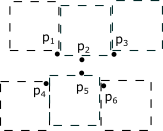
\includegraphics[width=0.4\textwidth]{A41a.png}
	\caption{ This is how to place the six positions. }
\end{figure}

As you can see the 4-slider model can place all six labels. 

\begin{figure}[H]
	\centering
	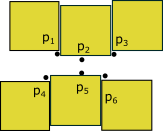
\includegraphics[width=0.4\textwidth]{A41b.png}
	\caption{The labels placed with the 4-slider model}
\end{figure}

The fixed position model can only place 4 labels, because the positions $(X,0)$ and $(Y,1)$ are not in the fixed position model.
Also I cannot move the labels to another position to the left or right, because then the label would overlap with the outer labels. 
 $ p_{5}$ cannot place it label between $p_{4}, p_{6}$, because it does not has position $(Y,1)$ and it cannot place it label between $p_{1}, p_{3}$, because it does not has position $(X,0)$.
\begin{figure}[H]
	\centering
	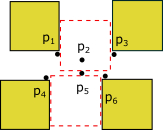
\includegraphics[width=0.4\textwidth]{A41c.png}
	\caption{The labels placed with the fixed position model}
\end{figure}

Even if I place on of the outer labels in the middle, I can only place 4 labels with the fixed position model, because it will overlap with the two other points in the middle.  
\begin{figure}[H]
	\centering
	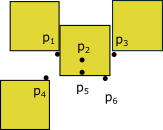
\includegraphics[width=0.4\textwidth]{A41d.png}
	\caption{The labels placed with the fixed position model}
\end{figure}

So I have shown that for any fixed position models, sometimes the 4-slider model  can sometimes label 1.5 times as many points. 

\bigskip

\exercise{2} 
I will use dynamic programming to solve the following problem:  Given a set  triangular cones $\Delta_1, \ldots \Delta_n$ I want to select active ranges $[0,A_1], [0,A_2], \ldots [0,A_n]$ such that $\sum_{i=1}^n A_i$ is maximized.
To do so, I have to divide the problem $A[i,j]$ in to multiple subproblems and I will need a function $height(a,b,c)$. 
First I will explain the function $height(a,b,c)$. The three inputs are three traingular cones. 
The output should be the maximum height of the first intersection of  $\Delta_c$ with $\Delta_b$ and $\Delta_a$. When there is no such intersection, the output should be Smax. 
So in the example of figure 5 $height(1,4,3)$ would return the height of the intersection between $\Delta_3$ with $\Delta_4$. 
 \begin{figure}[H]
	\centering
	
\includegraphics[width=0.4\textwidth]{A42a.png}
	\caption{A set of triangular cones.}
\end{figure}
For example I will show how to divide $A[1,3]$ in figure 5 in to multiple subproblems.
The maximum active range is the maximum of the following combinations: 
\begin{itemize}
\item $ height(0,4,1) + A[2,3]$
\item $A[1,1] + height(0,4,2) +  A[3,3]$
\item $A[1,2] + height(0,4,3) $
\end{itemize} 
I can now  see that the height is Smax ( suppose this is 4 in this example) for $height(0,4,1)$  and $ height(0,4,2)$ and around 3 for $height(0,4,3)$. 
Thus I now need to find the maximum of these combinations: 
\begin{itemize}
\item $4 + A[2,3]$
\item $A[1,1] +  3 +  A[3,3]$
\item $A[1,2] +  4$
\end{itemize} 
I now have to compute $A[1,2], A[1,1], A[3,3], A[2,3]$. 
For $A[2,3]$ I can do this by taking the maximum of the following combinations: 
\begin{itemize}
\item $ height(1,4,2) + A[3,3]$
\item $A[2,2] + height(1,4,3)$
\end{itemize} 
I can now see that $height(1,4,3)$ is still 3 and  $height(1,4,2)$ is still 4. 
I now have to compute $A[3,3]$ and $A[2,2]$, which are $height(2,4,3)$ and $height(1,3,2)$, which are both 2.5. 
Now I can see that  $A[2,3] = max \{ 6.5, 5.5\} = 6.5$ 
I can do the same for $A[1,2]$, which would result in 6.5. \\ 
So now the maximum for $A[1,3]$ becomes the maximum of : 
\begin{itemize}
\item $ 4  + 6.5$
\item $4 + 4 +  2.5$
\item $6.5 + 3 $
\end{itemize} 
Which is 10.5, which is exactly what I wanted. 
When I apply the algorithm to $A[0,4]$ I would get the following subproblems: 

Then I can find the maximum with the filled in dynamic table in figure 6. 
 \begin{figure}[H]
	\centering
	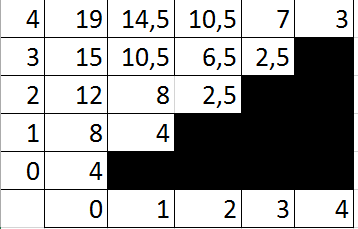
\includegraphics[width=0.4\textwidth]{A42b.png}
	\caption{The dynamic table for the set of triangular cones in figure 5.}
\end{figure}
The outcome of the algorithm for figure 5 is show in figure 7.
 \begin{figure}[H]
	\centering
	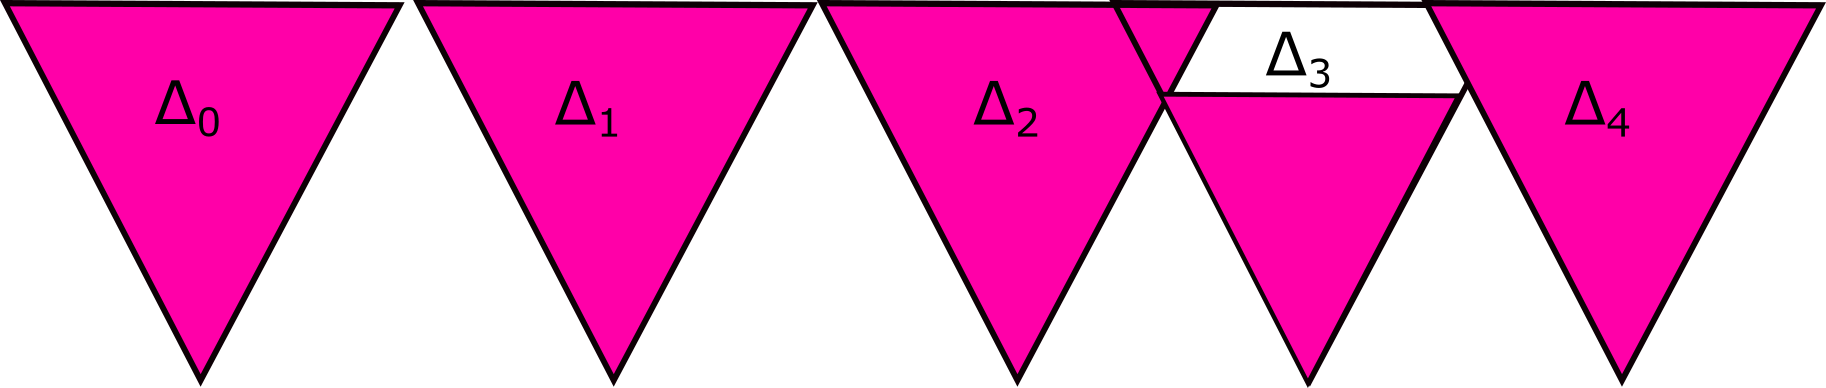
\includegraphics[width=0.4\textwidth]{A42c.png}
	\caption{The outcome of the algorithm for the set of triangular cones in figure 5.}
\end{figure}
So I can now define the subproblem generally : \\ 
$ A[i,j] = max \{ A[i,x] + \textit{height(i-1,j+1,x)} + A[x,j] \}$ , where $x$ is $i \leq x \leq j$. \\
Note that when I want to compute the height with a non existing triangular cone, such as -1 or n+1, I use a empty traingular cone and thus there is no intersection. \\
\textbf{Proof of correctness} \\ 
When I tried to proof the correctness of the algorithm I encountered a little problem in the algorithm. 
Normally the subproblems give optimal solutions and are thus used to formulate the proof, however the subproblems of the algorithm are influenced by $\Delta_{i-1}$ and $\Delta_{j+1}$ and are thus not necessary optimal solutions for the interval $i,j$. 
The algorithm solves $A[0,n]$ correctly, because that part is not influenced by $\Delta_{-1}$ and $\Delta_{n+1}$. 


\textbf{Running time} \\ 
 The algorithm has to compute $ A[i,j] $ where $ i \leq j \leq n$. 
 This are $ \frac{1}{2}n^2$ problems.
 For each problems the algorithm need at most $O(n)$ time, because the algorithm has to find the max of at most $n$ subproblems. 
 This would result in a total running time of $O(n^3)$.


\end{document}
